\begin{figure}[htbp]
    \centering
    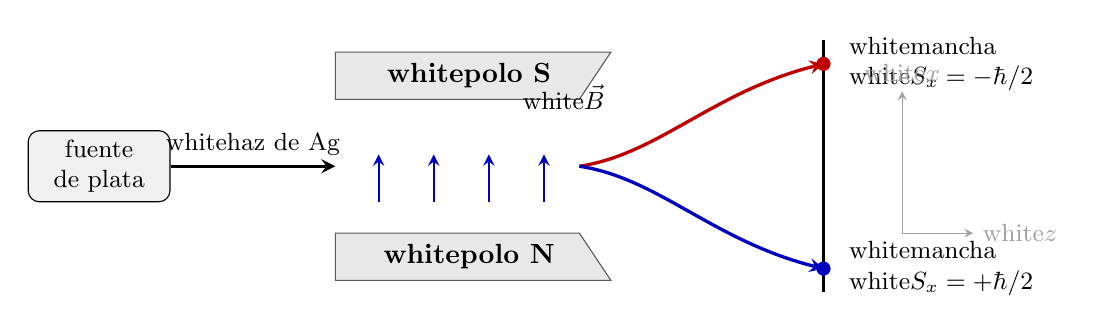
\begin{tikzpicture}[>=stealth, every node/.style={font=\small}]
        \node[draw,rounded corners,fill=gray!12,minimum width=1.8cm,minimum height=0.9cm,align=center] (source) at (0,0) {fuente\\de plata};
        \draw[->,very thick] (source.east) -- (3.0,0) node[midway,above] {\contour{white}{haz de Ag}};

        \draw[fill=gray!18,draw=gray!70!black] (3.0,1.45) -- (6.5,1.45) -- (6.1,0.85) -- (3.0,0.85) -- cycle;
        \draw[fill=gray!18,draw=gray!70!black] (3.0,-0.85) -- (6.1,-0.85) -- (6.5,-1.45) -- (3.0,-1.45) -- cycle;
        \node[font=\bfseries] at (4.7,1.15) {\contour{white}{polo S}};
        \node[font=\bfseries] at (4.7,-1.15) {\contour{white}{polo N}};
        \foreach \z in {3.55,4.25,4.95,5.65} {
            \draw[->,blue!75!black,thick] (\z,-0.45) -- (\z,0.15);
        }
        \node[above] at (5.9,0.6) {\contour{white}{$\vec{B}$}};

        \draw[->,very thick,red!75!black] (6.1,0) .. controls (7.1,0.15) and (7.8,0.95) .. (9.2,1.3);
        \draw[->,very thick,blue!75!black] (6.1,0) .. controls (7.1,-0.15) and (7.8,-0.95) .. (9.2,-1.3);
        \draw[very thick] (9.2,-1.6) -- (9.2,1.6);
        \fill[red!75!black] (9.2,1.3) circle (0.09);
        \fill[blue!75!black] (9.2,-1.3) circle (0.09);
        \node[right,align=left] at (9.4,1.3) {\contour{white}{mancha}\\\contour{white}{$S_x=-\hbar/2$}};
        \node[right,align=left] at (9.4,-1.3) {\contour{white}{mancha}\\\contour{white}{$S_x=+\hbar/2$}};
        \draw[->,gray!75] (10.2,-0.85) -- (10.2,0.95) node[above] {\contour{white}{$x$}};
        \draw[->,gray!75] (10.2,-0.85) -- (11.1,-0.85) node[right] {\contour{white}{$z$}};
    \end{tikzpicture}
    \caption{Analizador Stern--Gerlach con gradiente en la dirección $x$: $\vec{B}=B_x\vec{e}_x$ y $\partial B_x/\partial x>0$. La fuerza $\vec{F}=\mu_x(\partial B_x/\partial x)\vec{e}_x$ separa el haz según $S_x=\pm\hbar/2$; para el electrón, $\vec{\mu}_e$ es antiparalelo a $\vec{S}$.}
    \label{fig:sg-x}
\end{figure}